% CVPR 2022 Paper Template
% based on the CVPR template provided by Ming-Ming Cheng (https://github.com/MCG-NKU/CVPR_Template)
% modified and extended by Stefan Roth (stefan.roth@NOSPAMtu-darmstadt.de)

\documentclass[10pt,twocolumn,letterpaper]{article}

%%%%%%%%% PAPER TYPE  - PLEASE UPDATE FOR FINAL VERSION
\usepackage[review]{cvpr}      % To produce the REVIEW version
%\usepackage{cvpr}              % To produce the CAMERA-READY version
%\usepackage[pagenumbers]{cvpr} % To force page numbers, e.g. for an arXiv version

% Include other packages here, before hyperref.
\usepackage{graphicx}
\usepackage{amsmath}
\usepackage{amssymb}
\usepackage{booktabs}
\usepackage{enumitem}
\usepackage{float}

% It is strongly recommended to use hyperref, especially for the review version.
% hyperref with option pagebackref eases the reviewers' job.
% Please disable hyperref *only* if you encounter grave issues, e.g. with the
% file validation for the camera-ready version.
%
% If you comment hyperref and then uncomment it, you should delete
% ReviewTempalte.aux before re-running LaTeX.
% (Or just hit 'q' on the first LaTeX run, let it finish, and you
%  should be clear).
\usepackage[pagebackref,breaklinks,colorlinks]{hyperref}


% Support for easy cross-referencing
\usepackage[capitalize]{cleveref}
\crefname{section}{Sec.}{Secs.}
\Crefname{section}{Section}{Sections}
\Crefname{table}{Table}{Tables}
\crefname{table}{Tab.}{Tabs.}


%%%%%%%%% PAPER ID  - PLEASE UPDATE
\def\cvprPaperID{47} % *** Enter the CVPR Paper ID here
\def\confName{AI2100}
\def\confYear{2022}


\begin{document}

%%%%%%%%% TITLE - PLEASE UPDATE
\title{Explaining answers given by neural question answering systems}


\maketitle

%%%%%%%%% ABSTRACT
\begin{abstract}
Question answering has been a fundamental challenge in NLP with vast applications. State of the art neural question answering systems are able to beat humans at this task when evaluated on carefully prepared datasets. However it is difficult to explain in human comprehensible manner, how these models reach the answers that they do. Such an explanation is often important in high stakes situations such as healthcare or business applications. Thus we propose to explore explainability methods in the context of neural question answering through this project.
\end{abstract}

%%%%%%%%% BODY TEXT
\section{Further Literature Review}
To widen our understanding of the chosen problem, we did a further review of literature, this time, about explainability in NLP, with major emphasis on BERT model for Question Answering.


% start here
~\cite{mudrakarta:2018} proposes to use Integrated Gradients (IG) ~\cite{IG} for visual question answering, tabular question answering as well as reading comprehension to find input attribution scores. The model used for reading comprehension is an attention based model. This method guarantees that uninfluential variables will not get any attribution and helps us to identify weaknesses of the model which can be used to improve it.


BERT and its variants have achieved state-of-the-art performance on various NLP tasks, such as sentiment analysis, question answering, etc. Although transformers are believed to be moderately interpretable through the inspection of their attention values, ~\cite{at_not_exp} shows that this may not be the case always. 

~\cite{bert_layers_qa} proposes that the hidden states contain valuable information that can be leveraged to get interpretable results. They inspect how QA models transform token vectors, to find the answer. To that end, they apply a set of general and QA specific probing tasks to get an insight into internal representations in transformer layers. They also performed visualization of hidden representations, using dimensionality reduction techniques like PCA ~\cite{PCA} to get further insight. They show that transformations within BERT go through phases that are related to traditional pipeline tasks. These phases are also analogous to human reasoning processes. Also, they reveal that fine-tuning has little impact on models' semantic abilities and prediction errors can be identified in representations of early layers itself. 

    A similar work, ~\cite{bert_for_qa} attempts to interpret layer-wise functionality in BERT specifically for Reading Comprehension Question Answering (RCQA) task, using Integrated Gradients . They found that, the initial layers of BERT focus on query-passage interaction, while the later layers focus more on task specific functionalities such as contextual understanding, improving the answer predictions, etc. They also observed that, BERT focuses on confusing words in the later layers, but still manages to give the right answers.

The above two works show that, the initial layers of BERT capture general semantic meanings of words, while the middle layers extract the contextual relations, eventually helping the final layers to come up with the answers to the questions.

\section{Results reproduced from literature}
We fine-tuned a pre-trained Bert-base-uncased model from the huggingface library. We used the SQuAD 1.1 ~\cite{squad} dataset for fine-tuning. In this dataset, there are 87599 examples for training and 10570 examples for evaluation. Each example consists of a question and a corresponding context. 

The answer to each question is a contiguous phrase from the context itself. Therefore every answer can be represented as a start-position and an end-position with respect to the context. Thus it can be easily seen that we have reduced the task of question answering to the task of regression of two variables. In order to do this regression, a linear layer with two outputs is added on top of the Bert model. This model has already been implemented in huggingface library as BertForQuestionAnswering and was used from there.

The loss function used is the average of cross-entropy losses of start and end positions. Fine-tuning was done for 2 epochs. Total time taken was 4 hours on Tesla T4 GPU in Google colab. The optimizer used was AdamW~\cite{AdamW}. The final training loss was 0.779 and final validation loss was 1.016.

Huggingface APIs were taken full advantage of. The code can be found in the attached notebook: "bert-fine-tune.ipynb".

\section{Preliminary results}
We have used an uncased BERT model from the Hugging face library which is fine-tuned on the SQuAD-v1 to analyse the layer attributions. We used \textbf{Integrated Gradients} from \href{https://captum.ai/}{\textbf{Captum}} (an explainable AI toolkit) to compute the attribution scores for each word.
Integrated Gradients for a model $F$ and input $x_i$ is calculated as follows:
\begin{equation}
    \displaystyle IG(x_i) = \int_{0}^{1}\frac{\partial F(\tilde{x}+\alpha(x_i - \tilde{x} )}{\partial x_i} d\alpha
\end{equation}
We obtained the following results,\\

\begin{figure}[h]
    \centering
    \onecolumn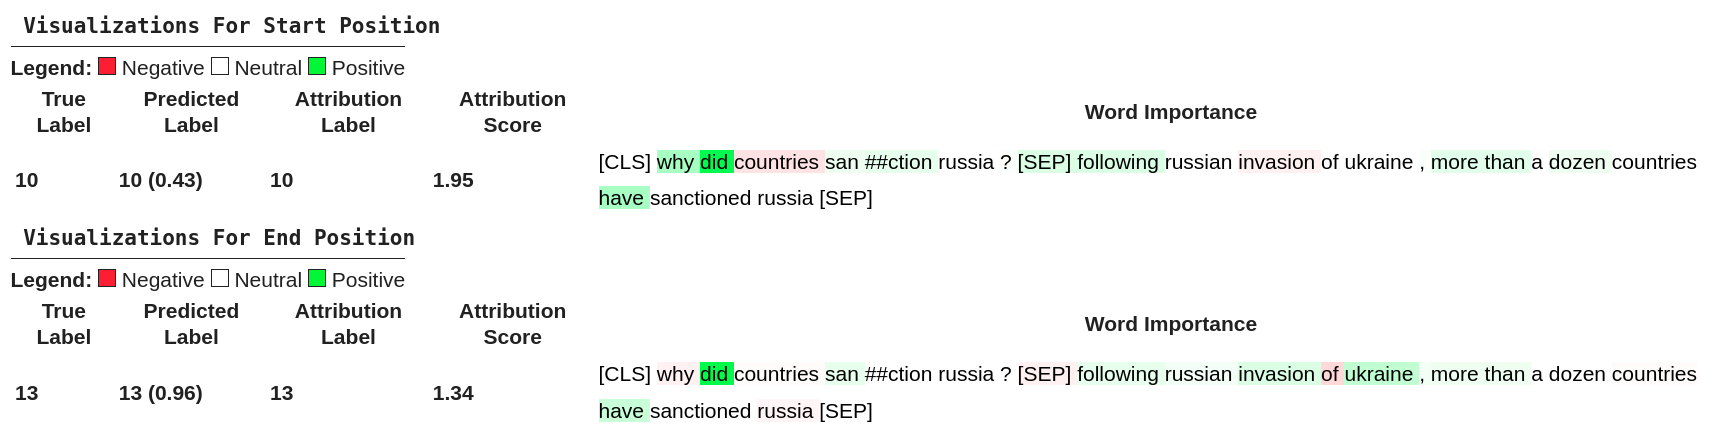
\includegraphics[width=\textwidth]{1.png}
    \caption{Visualization of attribution scores for each input word.}
    \label{fig:my_label}
\end{figure}


\centerline{\textbf{Predicted Answer :} russian invasion of ukraine}


\begin{figure}[ht]
    \centering
    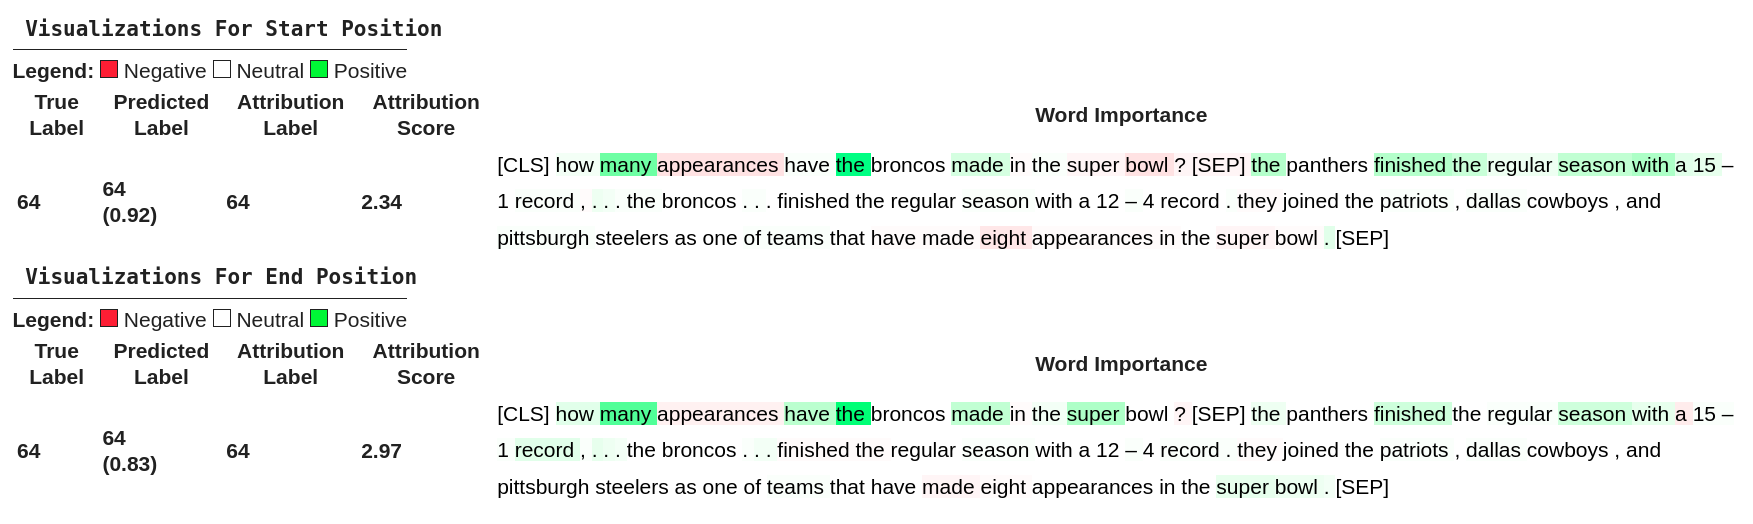
\includegraphics[width=\textwidth]{2.png}
    \caption{Visualization of attribution scores for each input word.}
    \label{fig:my_label}
\end{figure}
\centerline{\textbf{Predicted Answer :} eight }
\twocolumn
From the above results we can see that for predicting the start position of the answer, the model focuses more on the question and for predicting the end position of the answer, the model starts focusing on the context. The code for visualizing the attributions can be found in the attached notebook: "Attribution\_visualization.ipynb"

%%%%%%%%% REFERENCES
{\small
\bibliographystyle{ieee_fullname}
\bibliography{egbib}
}

\end{document}
